\chapter[Using Emotion Classification Models against Stack Overlow]
{Using Emotion Classification Models against Stack Overflow\pubfootnote{Graetsch:2021caise}}
\label{ch:caise2021}
\graphicspath{{mainmatter/publications/figures/caise2021/}}

\glsresetall
\begin{abstract}
Pre-trained \gls{ai} models are increasingly available as \glsacpl{api} and tool-kits to software developers, making complex \gls{ai}-enabled functionality available via standard and well-understood methods. However, reusing such models comes with risks relating to the lack of transparency of the model and training data bias, making it difficult to confidently employ the toolkit in a new situation.  Vendors are responding and proposing artefacts such as model cards and datasheets to make models and their training more transparent.  But is this enough?  As part of an empirical investigation determining if a cloud-based \glspl{iws} was ready for production use, we processed developer questions on \glslong{so} using a published pre-trained classifier that was specifically tuned for the software engineering domain. In this paper, we present lessons learnt from this automation effort. We found unexpected results which led us to delve into model and training data---an option available to us because the information was available for research.  We found that, had a model card and datasheet been prepared, we could have identified risks to our study much earlier on. However, model cards and datasheet specifications are not yet mature enough and additional tools and processes are still required to confirm a decision whether a trained model can be reused with confidence.
\end{abstract}
\glsresetall

\section{Introduction}
Pre-trained \gls{ai} models are increasingly available to software developers either directly or wrapped into web-based components and toolkits; for example, Google's Cloud \gls{ai}\footnoteurl{https://bit.ly/2VheoH2}{29 Nov 2020} or Microsoft Azure's Cognitive Services.\footnoteurl{https://bit.ly/37jiwvU}{29 Nov 2020} The grand promise is the rapid creation of \gls{ai}-infused functionality into end-applications as developers can simply reuse models instead of training them from scratch, as training is laborious and resource-intensive~\citep{RamanAnandHoder2015}. Vendors do provide usage guidelines, component documentation, code examples and a compelling marketing narrative, although the limitations and risks are not as well-presented in  official documentation~\citep{Cummaudo:2019icsme,Cummaudo:2020icse}. 
In practice, developers and technical architects study issue trackers and online forums such as \gls{so} to assess and inform their decisions.  Multiple studies highlight the value and insights to be gained from these online forums~\citep{Abdalkareem2017WhatOverflow,Storey2014,Cummaudo:2020icse}.

This work began as an investigation determining whether these services are production-ready for certain industry use cases (e.g., computer vision). Inspired by the possibility of finding insight from content in the online forums, we wanted to analyse the issues raised on \gls{so} by developers that relate to computer vision-based \glspl{iws}, i.e., \glspl{cvs}.  Although manual analysis is feasible for this task, we decided to use a pre-trained natural language processing technique for a more automated approach to understand developers' frustration. This was motivated by (i) the gain from automation---specifically having an efficient,  repeatable process and, more importantly, (ii) to learn about potential issues when using pre-trained models in a related, but new, contexts. \Cref{caise2021:sec:study} explains this in further detail.

In our analysis, beyond the direct summative aspects, we focused on emotions within the content posed on the online forums. This was motivated by work done by~\citet{wrobel2013}, who suggested that some negative emotions can pose risk to developer productivity. However, while anger is a negative emotion, it can (in some people) generate a motivating response \citep{wrobel2013}. Our goal was to determine whether negative emotions (and specifically, \textit{which} negative emotions) are the predominant theme within questions on these forums regarding \glspl{iws}.  The natural expectation is that developers would not pose questions unless they needed support and help, and we expected to find a high prevalence of anger-based emotion in the questions (frustration that the service is not working as they think should), and perhaps surprise at any unexpected behaviour. Similarly, we would expect the tone of responses to questions to be neutral, and hopefully supportive. Our focus, however, remains on the questions posed.

Our findings, elaborated further in \cref{caise2021:SubSection:Findings}, were surprising. While the pre-trained model we selected was trained specifically on \gls{so} and tuned for emotions~\citep{novielli2018,calefato2017}, our results show that 14\% issues were considered by the model with the positive emotions of \textit{Love} or \textit{Joy}, and only a surprisingly small amount (5\%) fell into \textit{Anger} (or frustration). A closer examination using multiple human reviewers showed an even more interesting insight: human reviewers did not agree with the automated machine classification, and worse, the reviewers did not agree with each other, suggesting that training machines with a consistent set of labels is a non-trivial exercise.  Finally, we reflected whether the pre-trained classifier could be better documented.  We found vendors are recognising these challenges and are offering solutions to better document their models~\citep{Mitchell:2018in, Gebru:2018wh}. However, when we looked into the information captured by these solutions, we found their specification to be very broad and additional guidance for completion is required to help evaluate risks faced in an industry context (discussed in \cref{caise2021:sec:disussion}). 

\section{Motivation}\label{caise2021:sec:study}

The initial context of our work was to explore reusable cloud-based \glspl{cvs},\footnote{Such as Google Cloud Vision, Azure Computer Vision, or Amazon Rekgonition} arising for use in an industry context on a client project. Our prior research has identified growth in questions on \gls{so} relating to such services~\citep{Cummaudo:2020icse}, thus enabling us to explore a rich dataset about developers' concerns about these pre-packaged and cloud-based \gls{ai}-components.

Aware that productivity of software developers can be adversely impacted by negative emotion \citep{wrobel2013}, we decided to explore the emotions within our dataset expressed by developers through the questions they pose on \gls{so}. Our intent was to identify whether developers are surprised, angry, frustrated, or overall positive about using these \glspl{cvs} (as expressed as emotions in their \gls{so} questions). This was motivated by prior work,  which shows that---despite their technical nature---\gls{so} questions do exhibit emotion~\citep{Novielli:2015vda, calefato2017}.  Although we could have read these posts manually, for consistency, repeatability, and efficiency, we chose to automate this process by utilising an emotion-aware text classification system trained specifically on \gls{so} data \citep{novielli2018}. Our expectation was that we would gain some insight into the questions through the emotions, and we hypothesised that we would see a high proportion of surprise (i.e., the \glsac{api} does not work as expected) and anger (frustration due to mismatched expectations).

%The  goal of our study was to assess the feasibility of utilising automated emotional text classification of developer questions in \gls{so} to support downstream prioritisation of questions for issue resolution and perform further analysis.  

To permit replication, the raw results produced from this case study are made available online at \url{https://bit.ly/3eSp7ku}.

\section{Method}\label{caise2021:sec:method}
We selected a classifier included in the EMTk toolkit that was specifically trained for emotional text classification in the software engineering domain~\citep{calefato2017}. The EMTk toolkit is available with a fully labelled training dataset~\citep{novielli2018}, permitting reuse and analysis of internals.  The classifier is based on \citeauthor{shaver1987}'s emotional hierarchy model~\citep{shaver1987} and performs binary classifications against text data provided in input files and an input parameter designating the emotion to be classified---one of \textit{Love}, \textit{Joy}, \textit{Surprise}, \textit{Fear}, \textit{Sadness} or \textit{Anger}. The classifier utilises \gls{svm} classification and a \gls{dsm} built using Word2Vec. This model is trained on 20 million \gls{so} posts. The \gls{dsm} approach facilitates classification to take into consideration the surrounding context of the word, in addition to the polarity of individual words~\citep{calefato2018}.   


As input for the classifier, we used a dataset of 1,425 \gls{so} questions restricted to intelligent \glspl{cvs}, available from~\citet{Cummaudo:2020icse}.  We ran the classifier with the same input dataset for each of the six emotions.
%\begin{figure}
 %   \centering
  %  \includegraphics[width =0.5\textwidth]{Diagram4.png}
  %  \caption{Our Method}
  %  \label{caise2021:fig:our method}
%\end{figure}
To cross-check classified output, we manually annotated a random sample of 300 questions with zero or more of the six emotions. Each of these 300 posts were assigned to three raters who individually carried out the following three steps: (i) identify the presence of emotion(s); (ii) if emotion(s) exists, classify the emotion(s) under one or more of the six basic emotions as per the Shaver framework. The coding guidelines provided by \citet{novielli2018} were adhered to to assist with emotion classification per post.  After collating each rater's results, we calculated a Fleiss' Kappa~($\kappa$)~\citep{Fleiss:1971ff} as a measure of inter-rater agreement per emotion for each of the three human raters (manual rating), using the \texttt{irr} computational R package~\citep{Gamer:tj} per suggestions provided in~\citep{Hallgren:2012kt}. Once completed, the three raters discussed discrepancies between posts classified with different emotion where agreement for that emotion was low, however we did not change any emotions that were initially assigned as this would impact reliability of our interpretation of \citet{novielli2018}'s guidelines. We then used the results from the classifier as a `fourth' \textit{automated} rater, comparing the results with the manual rating by calculating the agreement for each emotion and Fleiss' Kappa for further inter-rater agreement analysis.

%\subsection{Results} \label{caise2021:SubSection:Findings}
Of the 1,425 \gls{so} questions, the classifier did not classify any emotion in 622 posts (labelled \textit{No Emotion}). The remaining posts were classified as: 224 posts as \textit{Fear}, 223 as \textit{Surprise}, 70 as \textit{Sadness}, 103 as \textit{Love}, 100 as \textit{Joy}, and 76 as \textit{Anger}. Some posts were classified against two or more emotions, and as a result, the total proportions do not add up to exactly 100\%. See \cref{caise2021:tab:emotion-freqs}.  Results from our inter-rater analysis are reported in \cref{caise2021:tab:reliability-analysis}.


\begin{table}
    \caption[Emotion classification frequencies]{Emotion classification frequencies.}
    \centering
    \label{caise2021:tab:emotion-freqs}
    \small
    \begin{tabular}{l|cc}
    \toprule
    \textbf{Emotion}&
    \textbf{Frequency}&
    \textbf{Proportion}\\
    \midrule
   Love&103&7.2\%\\
   Joy&100&7.0\%\\
   Surprise&223&15.6\%\\
   Sadness&70&4.9\%\\
   Fear&224&15.7\%\\
   Anger&76&5.3\%\\
   No Emotion&622&43.6\%\\
    \bottomrule
    \end{tabular}
    \end{table}
   \begin{table}
   \caption[Reliability Analysis of Emotion Classification]{Results from Inter-Rater Agreements.}
   \centering
   \label{caise2021:tab:reliability-analysis}
   \small
   \begin{tabular}{l|cc}
   \toprule
   \textbf{Emotion}&
   \textbf{Three Raters}&
   \textbf{Three Raters + Classifier}\\
   \midrule
   Love&0.13~~\textit{(slight)}&0.19~~\textit{(slight)}\\
   Joy&0.23~~\textit{(fair)}&0.13~~\textit{(slight)}\\
   Surprise&0.15~~\textit{(slight)} &0.11~~\textit{(slight)}\\
   Sadness&-0.01~~\textit{(poor)}&0.00~~\textit{(poor)}\\
   Fear&0.25~~\textit{(fair)}&0.07~~\textit{(slight)}\\
   Anger&0.05~~\textit{(slight)}&0.04~~\textit{(slight)}\\
   No Emotion&0.09~~\textit{(slight)}&0.10~~\textit{(slight)}\\
   \bottomrule
   \end{tabular}
   \end{table}

Guidelines of indicative strengths of agreement are provided by~\citet{Landis:1977kv}, where: $\kappa \leq 0$ indicates \textit{poor} agreement; $0 < \kappa \leq 0.2$ indicates \textit{slight} agreement; $0.2 < \kappa \leq 0.4$ indicates \textit{fair} agreement; $0.4 < \kappa \leq 0.6$ indicates \textit{moderate} agreement; $0.6 < \kappa \leq 0.8$ indicates \textit{substantial} agreement. These interpretations suggest that, when using the classifier's output as a fourth `rater', there was slight agreement on all emotions except \textit{Sadness}, where agreement was poor.  Agreement amongst the three human raters was slight for \textit{Love, Surprise, Anger and No Emotion}, fair for both \textit{Joy and Fear}, and poor for \textit{Sadness}. 

\section{Results}\label{caise2021:SubSection:Findings}
In this section, we present our findings with respect to limitations in the classifier and our investigation of the dataset that was used to train the classifier. Given the weak results, we then  discuss whether model cards~\citep{Mitchell:2018in} and/or datasheets~\citep{Gebru:2018wh} could have provided a more effective approach to informing the viability and limits of the pre-trained model.

\subsection{Limitations of the Text Classifier}
The classifier did not assign any emotion to more than 43\% of the \gls{so} posts.  This result corroborates the findings by~\citeauthor{murgia2014}, who identified via a manual process \textit{No Emotion} as the most prevalent classification~\citep{murgia2014}. For illustration, we provide a set of examples in \cref{caise2021:tab:example-so-questions}. (The ratings column indicates the emotion labels assigned by each of the three human raters $R_{1..3}$ and the label assigned by the classifier $C$.) 
The first example given in \cref{caise2021:tab:example-so-questions} illustrates a neutral example, where none of the raters, including the classifier identified any emotion.  
In the second example, the classifier did not detect any emotion, however all three human raters agreed that the question indicated \textit{Sadness}. 
In the third example, each rater identified different emotions, thereby indicating complete disagreement.
In the fourth example, the classifier interpreted the question as \textit{Joy}, whereas the human raters identified \textit{Surprise} and \textit{Anger}. Whilst that question had a word typically associated with \textit{Joy} (i.e., ``I'm \uline{pretty} sure...''), the realistic context here is that the phrase `pretty' indicates no emotion and the wider context of the question shows how the human raters identified a sense of frustration (anger) and surprise at the results the developer is finding.
Lastly, two, additional examples are presented in the last and second-last rows of \cref{caise2021:tab:example-so-questions} to highlight different inconsistencies both between human raters and the classifier.

\afterpage{\begin{landscape}
\begin{table} 
\caption[Sample questions comparing automated and human rater classifications]{Human Raters (\textit{R1, R2, R3}) versus automated classifier (\textit{C)}. Questions located at: https://stackoverflow.com/q/[ID].}
\label{caise2021:tab:example-so-questions}
\centering
\tablefitlandscape{1}{\begin{tabular}{p{.9\linewidth}  p{0.2\linewidth}}
\toprule
\textbf{Question ID and Quote}&
\textbf{Ratings}\\
\midrule
{\textbf{[42375271]}~\textit{``Can we use Microsoft Emotion API in our Android Apps, considering the fact that it's still in its 'Preview' mode...can we create our own customized app using the code of EMOTION API to recognize the moods of users in our own app?''}}&
[$C$]:~No Emotion\newline
[$R_{1}$]:~No Emotion\newline
[$R_{2}$]:~No Emotion\newline
[$R_{3}$]:~No Emotion\\
\midrule
{\textbf{[55599305]}~\textit{``I have consumed the google cloud vision api to recognize a document with a table, but sometimes the image will be a little rotated, im triyng to get the value using theof the key i want, but how do i get it if it's not on the same.I was thinking of making a 'line' above and below the and finding if the point is between that, but i dont know how to do it.''}}&
[$C$]:~No Emotion\newline
[$R_{1}$]:~Sadness\newline
[$R_{2}$]:~Sadness\newline
[$R_{3}$]:~Sadness\\
\midrule
\textbf{[43534783]}~\textit{``Can someone try Google VisionAPI FaceTracker and see if it works? ...All I get when I try running it is a black screen (after fixing). I don't get any errors in the logs either.''}&
[$C$]:~Fear\newline
[$R_{1}$]:~Surprise\newline
[$R_{2}$]:~No Emotion\newline
[$R_{3}$]:~Anger\medskip\\
\midrule
\textbf{[51444352]}~~\textit{``I'm pretty sure I set up my IAM role appropriately (I literally attached the ComprehendFullAccess policy to the role) and the Cognito Pool was also setup appropriately (I know this because I'm also using Rekognition and it works with the IAM Role and Cognito ID Pool I created) and yet every time I try to send a request to AWS Comprehend I get the error... Any idea of what I can do in this situation?''}&
[$C$]:~Joy\newline
[$R_{1}$]:~Surprise\newline
[$R_{2}$]:~Surprise\newline
[$R_{3}$]:~Anger\medskip\\
\midrule
\textbf{[50190527]}~\textit{``I am trying to perform OCR on pdf documents using google cloud vision API, i uploaded a pdf document into a cloud bucket and downloaded the oauth key file and added it in the script as below. But when i run the file, i get the permission denined: 403 error, can anyone please give me instructions on how to fix it, i did extensive google search and did not yield any results, i am surely missing something here... I have checked the older stack overflow questions and the links provided in answers are not active anymore.Thanks in advance for your help.''}&
[$C$]:~No Emotion\newline
[$R_{1}$]:~Sadness\newline
[$R_{2}$]:~No Emotion\newline
[$R_{3}$]:~Anger\medskip\\
\midrule
{\textbf{[48145425]}~\textit{``I am Deploying Google cloud vision Ocr in My angular2 webapp. but i am getting many of the errors when i add this code in my webapp code. please help me to sort out this.''}}&
[$C$]:~Fear\newline
[$R_{1}$]:~Fear\newline
[$R_{2}$]:~No Emotion\newline
[$R_{3}$]:~Sadness\\
\bottomrule
\end{tabular}}
\end{table}\end{landscape}}

%\subsection{Peering into the Training Dataset}
We investigated our training dataset and related research documentation to see if that would give us further insights.  We found two areas warranting further exploration---training data balance and training data annotation. 

\subsection{Data imbalance}
 We found that the purpose of the training dataset was actually to train two classifiers---a sentiment classifier and an emotional classifier.  Each post in the training dataset was labelled with zero, one or more emotions. In addition, emotions were grouped, i.e., the positive emotions of \textit{Joy} and \textit{Love} were grouped into positive sentiment while \textit{Sadness}, \textit{Anger} and \textit{Fear} were grouped into negative sentiment. \textit{Surprise} was assigned either positive or negative sentiment, depending on context~\citep{novielli2018, calefato2018}.  \Cref{caise2021:fig:data-imbalance-training} shows the distribution of emotion labels across 4,800 posts in the training dataset; \textit{No Emotion} ($n=1959$) is removed to emphasise emotion-only results. Note: some posts in the training data set were classified as more than 1 emotion, hence the total counts add up to greater than 4800.

\begin{figure}
    \centering
    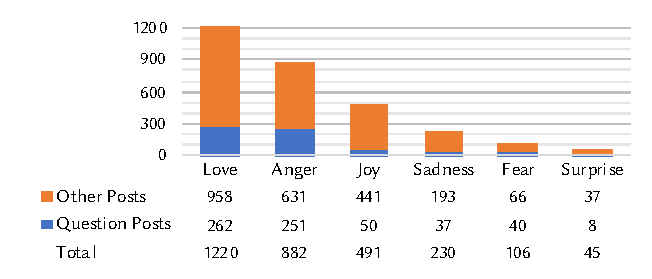
\includegraphics[width=.8\linewidth]{data-imbalance.pdf}
    \caption [Emotion classifier training data imbalance]{The emotion classifier training dataset distribution is largely skewed toward \textit{Love}, resulting in data imbalance. (\textit{No Emotion} labels were removed from this graph.)}
    \label{caise2021:fig:data-imbalance-training}
\end{figure} 

Class imbalance and its impact on classifier models is a known problem in \gls{ml}~\citep{Lopez2014, Weiss2004}, where  one class (known as the majority, positive class) significantly outnumbers the other class (known as the minority, negative class).  The impact of class imbalance on classification models results in minority classes with lower precision and lower recall than the majority class, since the classifier does not generate rules for the minority class.  One set of relevant techniques for addressing class imbalance is data sampling; including undersampling or subsampling, oversampling and hybrid approaches~\citep{Lopez2014}.
Whilst the training dataset seems balanced for the purpose of sentiment analysis, there is a lack of balance across individual emotions.  The predominant emotion in the training dataset was \textit{No Emotion} at 40.8\% of total posts. The most dominant emotions were \textit{Love} and \textit{Anger} at 25\% and 18\% respectively.  Less than 1\% of posts were labelled with \textit{Surprise}.  This means that the number of posts falling into some of the categories, for example, \textit{Surprise} and \textit{Fear} (i.e., 45 and 106 posts, respectively) is very low for training purposes. 

Further, the training dataset was spread across different types of \gls{so} posts (i.e., questions posts, answer posts, question comments, answer comments) to capture the different emotional language, however our study was interested in classifying \gls{so} question posts only. Of the training dataset's 4,800 posts, only 1,044 could be identified as question posts and within that subset of posts, the distribution of emotions was more polarised than in the overall 4,800 posts. \textit{Love} and \textit{Anger} are the most predominant emotions in the training dataset, however \textit{Anger} has a higher proportion (24\%) in question posts, as opposed to only 18.4\% in the overall dataset. 

In summary, the training dataset was not balanced within each emotion category and some emotions had very low sample numbers, as emphasised in the skew in \cref{caise2021:fig:data-imbalance-training}.  Proportions of training data examples per question per emotion was very low for \textit{Joy}, \textit{Surprise}, \textit{Sadness} and \textit{Fear}.
To address this imbalance and achieve better performance, training data could be enhanced to include additional samples or to use an oversampling approach.  A recent study into class-balancing approaches in the context of defect prediction models found that class rebalancing does lead to a shift in the learned concepts~\citep{Turhan2012OnModels}.

\subsection{Emotion Labeling Bias}\label{caise2021:SubSubSection:EmotionLabelingBias}
In software engineering, hierarchical categorical emotional frameworks---including those featured in \citet{Parrott2001}, \citet{Ekman1978} and \citet{shaver1987}---have been assessed by researchers and pragmatically selected as the basis for training emotional classifiers.  The chosen emotion framework is then used as the taxonomy of truth labels for classifier training datasets.  Data for labeling is sourced from systems such as \gls{so} and JIRA~\citep{murgia2014, ortu2016, gachechiladze2017, novielli2018}.  In the software engineering domain, truth labeling of emotions has, to date, been done manually~\citep{murgia2014, novielli2018, gachechiladze2017}.  Emotion annotation involves at least a pair of annotators~\citep{Ghazi2010HierarchicalTexts, Aman2007IdentifyingText}. For the EMTk training dataset, annotation was performed manually by a team of 12 coders, divided into four groups of three with a computer science background~\citep{calefato2017, novielli2018}.  Manual annotation challenges when coding emotions can be encountered due to different levels of semantic ambiguity within emotions and how humans express emotions in text~\citep{Hasan2014UsingMessages}. 

In the absence of an objective emotional truth, researchers' consistency is taken as a measure of correctness---i.e., multiple annotators that agree~\citep{murgia2014}.  A measure of inter-rater agreement is Cohen's Kappa~\citep{Cohen:1960tf} (for two raters) or  Fleiss' Kappa~\citep{Fleiss:1971ff} for more raters.  For the training dataset, inter-rater agreement ranged from $\kappa=0.30$ (fair) for \textit{Joy} to $\kappa=0.66$ (substantial) for \textit{Love}.  The researchers specifically trained dataset coders for consistency. The challenge of this approach with a subject such as emotions is the opportunity for bias.  In contrast, in other studies that used annotation, researchers specifically attempted to reduce the opportunity for biases by including raters with different nationalities, skills, cultural backgrounds, by increasing the number of raters~\citep{ortu2016} and opting against consistency training~\citep{Alm2005EmotionsText}.  As such, the approach taken to achieve consistency and makeup of label coders is important information for downstream consumers of an \gls{ai} model.

\subsection{Emotion Labelling and Classification Granularity}
Training data annotation was performed on \gls{so} posts---which included questions, answers, and comments to questions and answers.
Emotion annotation can be performed at different levels of granularity---word level~\citep{StrapparavaWordNet-Affect:WordNet}, spans of words in a sentence~\citep{Aman2007IdentifyingText}, sentence level or larger.  While a word level or keyword approach is considered too granular (as it does not capture the emotional context sufficiently), there is a risk of emotion progression during narratives and also within sentences~\citep{Aman2007IdentifyingText, murgia2014}.  Our \gls{cvs} dataset consisted of questions only as we were seeking to assess developer emotion expressed at the time of raising the question.  Question posts are typically longer than comments and may contain multiple emotions expressed at different levels of intensity that are interpreted differently by different readers.  

For example,  see the fifth question in \cref{caise2021:tab:example-so-questions}. We see that the first sentence does not carry any emotion, as the author is stating the steps to reproduce their issue. However, in the second sentence---where the \glsac{api} generates a ``403 error''---the author expresses a mix of both \textit{Sadness} and \textit{Anger} (i.e., frustration) since their ``extensive google search'' yielded no results, for which they begin to self-doubt (``i am surely missing something here''). Lastly, \textit{Love} is demonstrated in the last sentence, via appreciation in advance for potential responses to their question.

\section{Discussion} \label{caise2021:sec:disussion}

%\subsection{Using New tools: Model Cards and Datasheets}\label{caise2021:subsec:ModelCards}

There is a growing trend emerging from key industry vendors to better document pre-trained models using various means. For example, Google has proposed model cards to communicate performance characteristics of pre-trained models~\citep{Mitchell:2018in}.  Google has also published sample model cards relating to their Cloud Vision \glsac{api} for face and object detection\footnoteurl{https://bit.ly/2IXDLel}{28 November 2020} and, more recently, released a model card tookit\footnoteurl{https://bit.ly/3k7rLnk}{28 November 2020} to encourage other \gls{ml} practitioners to produce their own. Furthermore, this toolkit is now integrated into the Python library \texttt{scikit-learn} to help developers automatically generate model cards.\footnoteurl{https://bit.ly/36bXnEK}{28 November 2020} Microsoft has focused on a standardised process of dataset documentation through datasheets to encourage transparency and accountability by documenting the motivation, composition, collection process and intended uses of data~\citep{Gebru:2018wh}. This is a key building block of the `Responsible \gls{ml}' initiative led by the partnership on \gls{ai},\footnoteurl{https://bit.ly/33kebYc}{28 November 2020} which aims to increase the transparency of \gls{ai} and accountability of \gls{ml} system documentation.\footnoteurl{https://bit.ly/3lf8WPD}{28 November 2020} Lastly, IBM too has proposed a `FactSheet' concept combining model and data information~\citep{Arnold2019FactSheets:Conformity}.  

These tools are being adopted by organisations and researchers;  for example, Open \gls{ai} has published a basic model card of their generative language model\footnoteurl{https://bit.ly/3o6ECsj}{30 November 2020} and Google provided a sample model card for its toxicity analyser in its model card proposal paper~\citep{Mitchell:2018in}.  Model cards are also being considered for high stakes environments such as clinical decision making~ \citep{Sendak2020PresentingLabels}, where they facilitate overarching governance regimes on how and when models can be used.

In our case study, the combination of a model card for the classifier as well as a datasheet for training data would have provided valuable, easy to digest, and initial support to help evaluate whether the classifier is right for our context.  However, the current specification of datasheet contents is very broad and lacks detailed directions for those completing required information.  The model cards proposed by Google are focused on performance characteristics and do not sufficiently focus on the underlying data that was used to train and, hence, define the context of the classifier.

Had all the required information been provided to sufficient detail, including a highlight of the importance of rater consistency training, we could have better assessed risks and clarified at the outset whether an automated emotion assessment was an appropriate exercise. Further, with this information, we would be able perform our study with an more extensive rater consistency training, as well as a better appreciation of the limits of the classifier. 

{Hence, model cards and datasheets present rich opportunities for improving confidence and understanding in pre-trained \gls{ai} technology.} Now that toolkits are becoming increasingly available to make it easier for developers to generate toolkits, we suggest further research to evaluate model cards and datasheets (and combinations of the two) before pre-trained models are selected for specific tasks. This would make a valuable case study which we leave open for future work. Further, development of guidelines for model cards and datasheet creation, use and maintenance based on empirical evidence is also largely missing in literature; another avenue for potential research especially for use in industry contexts. A key challenge identified by this case study was the difficulty of validating results of an emotional classifier.  An additional research study could aim to capture developer emotion directly as they log questions and facilitate learning of developer emotion classification through this direct method (e.g., a think-aloud study).  This proposed approach to capturing data may shed further light into the emotional state an individual developer is experiencing \textit{as they write} their questions. However, it would be of interest to assess if it is possible to draw conclusions about emotions that developers feel \textit{in general}, due to the subjective nature of emotion.  That is, it is possible that different developers would report a range of emotions even when they write similar posts.

Once validation of the results can be improved, additional improvement could be considered for the EMTk classifier including training it on questions only and using some of the identified data balancing techniques to re-balance the dataset. Another area of potential research is whether providing feedback to developers about the emotional content in their posts would change what they communicate. For instance, would it assist developer productivity if they were made aware of the emotional content of their contributions/posts?   

\section{Threats to Validity} 

This case study represents only one detailed example of a classifier trained on the emotional model proposed by \citet{shaver1987}, documented in academic articles aimed to support research \citep{Novielli:2015vda, novielli2018, calefato2017, calefato2018}.  This impacts the external validity of our study as the results cannot be generalised to other domains or emotion classifiers. To mitigate this, it would be very useful and informative to compare and validate our findings across a number of classifiers, however this is challenging since there is generally a lack of detailed information (i.e., model cards and datasheets) for available classifiers to support the analysis. This said, even a simple comparative analysis of emotion classification outputs is difficult because emotional classifiers are typically trained on a specific emotional model. A mapping between emotional models would therefore be needed, which demands expertise beyond software engineering research.

Another key limitation is that our analysis focused on \gls{so} questions on a particular topic, whereas the EMTk had been trained on a mixture of different posts and topics. This again impacts the external validity of our results. It is not appropriate to draw a general conclusion from this analysis that emotions cannot be reliably classified by analysing text. In fact, there were higher inter rater scores achieved for EMTk's training dataset. Possibly additional rounds of clarification and moderation would yield a higher score and higher confidence.

It is common for questions on \gls{so} to be duplicates or downvoted, typically due to poor wording or a lack of detail in the body of the question. Duplicate and downvoted questions were not removed from our dataset used in the experiment, and, furthermore, any poorly worded questions may have impacted the automatic classifier's emotion labelling. This is likely to have impacted the measurement of our results.

\section{Related Work}

Emotion detection from text has been explored by researchers in depth. A recent survey of approaches, including the different emotion models and computational approaches, can be found in \citet{Sailunaz2018a} and \citet{Alswaidan2020}. Recently, researchers have also explored deep learning, specifically bidirectional BLSTM models, to improve emotion detection from text \citep{Batbaatar2019}.  Most approaches are supervised learning based, and hence rely on a labelled dataset for training.

Some related work of special interest has been done in the area of sentiment analysis, where discussions touched on emotion recognition. \citet{Novielli:2015vda} investigated the suitability of using sentiment analysis tools to measure affect in \gls{so} questions and comments.  In their analysis, they discussed that developers expressed negative emotions associated with their technical issues and that developers mainly express their frustrations for not being able to solve a problem. For questions with positive sentiment, they found that the positive lexicon did not express emotions, but rather positive opinions and use of positive speech acts associated with politeness and gratitude in advance of receiving a response.  Also, of interest is the evaluation of sentiment analysis tools evaluated on \gls{so}, JIRA and App Review datasets by \citet{lin2018sentiment}.  This study found that the prediction accuracy of the tools that were evaluated were biased against the majority class (neutral emotion).

The use of biometric sensors is also an area of active research for software developer emotion recognition.  This includes conducting experiments with correlated sensor data analysing the emotions software developers present whilst working \citep{Girardi2020}.  Further work could include using the biometric-based data as a data source for truth labels for emotion analysis as developers write their questions on \gls{so}, supporting the proposed studies mentioned in \cref{caise2021:sec:disussion}.

\section{Conclusion}\label{caise2021:sec:conclusion}
We started this work with an idea to use existing \gls{ai} techniques to \textit{automatically} investigate what other developers think of cloud \glspl{iws}. This translated into our attempt to use a  pre-trained model that learnt from posts provided by software engineers on \gls{so}. Developers learn, improve and deepen their skills from documentation, formal or self-paced education, experience, and sharing their knowledge. Good documentation often forms the foundation that enables learning and also to create educational aids. 

In this paper, we presented an observation case study that highlights a set of gaps in how a peer-reviewed model, published in the field of software engineering, lacks information about the limitations both within the documentation, as well as the articles published. To resolve these gaps, we investigated if new solutions that are being proposed (such as model cards) would have been of use to us before conducting our experiment. Model cards and datasheets will be a necessary and helpful first step, but as such we found their specification to be insufficient and additional guidance is required for those documenting the models cards and datasheets. Although we study only one pre-trained model in depth, our analysis shows that there are gaps in proposed solutions that can be addressed, and our future work will focus on investigating other models and \glspl{iws} to develop a more detailed documentation approach, specifically those that are being aimed for software engineering. 